\section{Questão 2}

Uma aplicação que permita ver equipas de futebol necessita de poder mostrar informações de um jogador especifico, informações de um treinador especifico, ou informações de uma equipa. Como se trata de uma base de dados doumental todas as informações associadas á equipa devem ser incluidas como documentos aninhados no documento da mesma, neste caso treinador e jogadores devem ser incluidos.
Assim a base de dados NoSQL MongoDB deverá ter 3 coleções, nomeadamente clube, jogador e treinador. Os documentos a produzir para cada coleção detalham-se em seguida com um exemplo:
\begin{enumerate}
	\item Clube
		\begin{figure}[H]

		  \centering
		  \captionsetup{justification=centering}

		  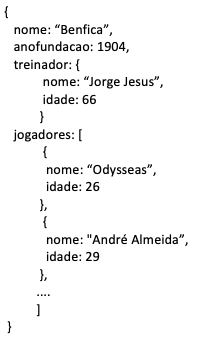
\includegraphics[scale = 0.5]{clube.png}
		  
		  \caption {Documento referente a um clube}
		\end{figure}
	\item Jogador
		\begin{figure}[H]

		  \centering
		  \captionsetup{justification=centering}

		  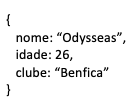
\includegraphics[scale = 0.5]{jogador.png}
		  
		  \caption {Documento referente a um jogador}
		\end{figure}
	\newpage
	\item Treinador
		\begin{figure}[H]

		  \centering
		  \captionsetup{justification=centering}

		  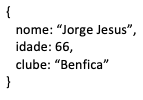
\includegraphics[scale = 0.5]{treinador.png}
		  
		  \caption {Documento referente a um treinador}
		\end{figure}
\end{enumerate}


\par Nota: Como para mim não é claro se devo ou não implementar a base de dados em MongoDB devido á questão 3 que se transcreve em seguida "Identifique as principais diferen\c{c}as da base de dados relacional acima descrita e a \textit{construida na alínea acima.}", decidi implementar a base de dados em Mongo para além de indicar a estrutura dos documentos.
\newline


\par Assim a base de dados foi criada e povoada recorrendo aos comandos listados no seguinte script. 

\begin{figure}[H]

  \centering
  \captionsetup{justification=centering}

  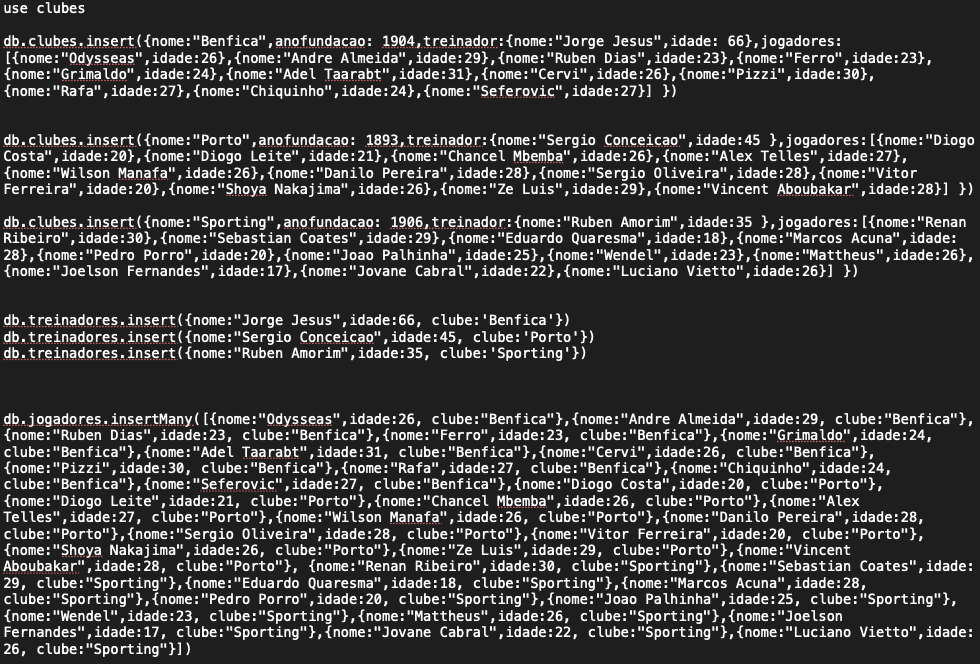
\includegraphics[width = \textwidth]{povoamentoMongo.png}
  
  \caption {Comandos usados para o povoamento da base de dados MongoDB}

  \label{fig:povoamento}
\end{figure}


\par A base de dados preenchida pode ser vista nas seguintes imagens.

\begin{figure}[H]

  \centering
  \captionsetup{justification=centering}

  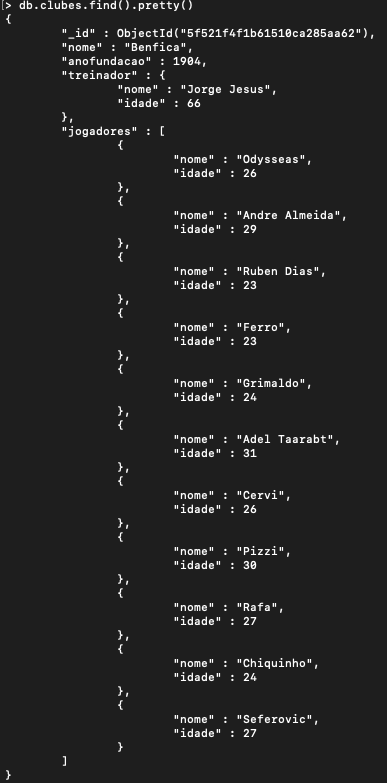
\includegraphics[width = 0.4\textwidth,height = 10cm]{clubes1.png}
  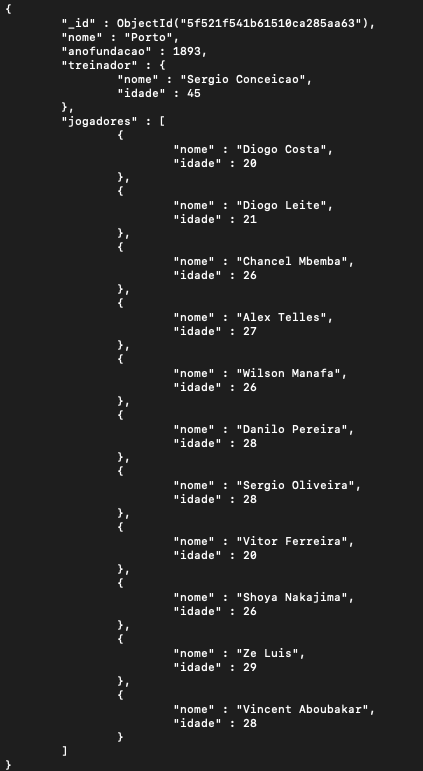
\includegraphics[width = 0.4\textwidth,height = 10cm]{clubes2.png}
  \caption {Documentos relativos aos clubes Benfica e Porto com a informação associada aninhada em subdocumentos}
  
  \vspace{0.5cm}
  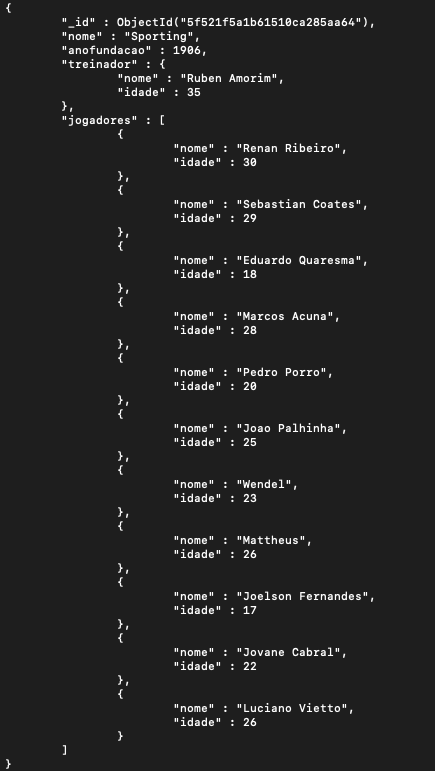
\includegraphics[width = 0.4\textwidth,height = 10cm]{clubes3.png}
  
  \caption {Documento relativo ao clube Sporting com a informação associada aninhada em subdocumentos}

  \label{fig:povoamento2}
\end{figure}

\begin{figure}[H]

  \centering
  \subfloat{{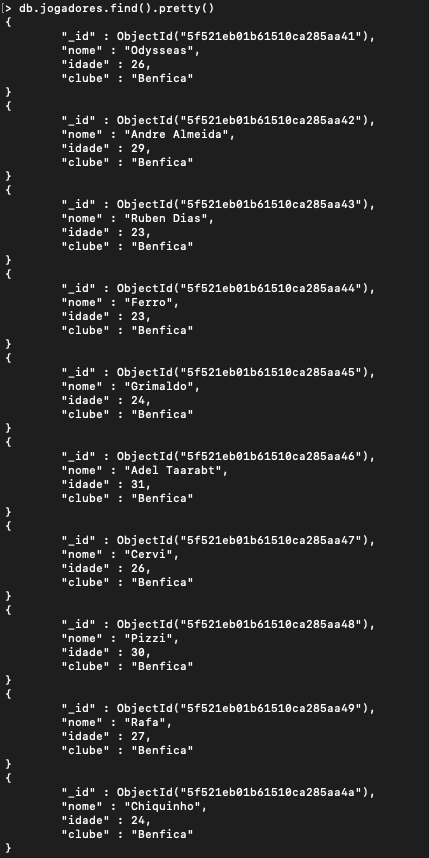
\includegraphics[width=.4\linewidth,height = 10cm]{jogadores1.png}}}
  \qquad
  \subfloat{{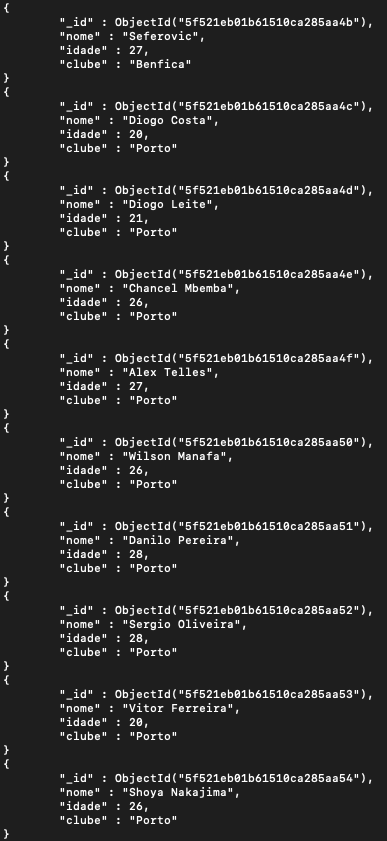
\includegraphics[width=.4\linewidth,height = 10cm]{jogadores2.png}}}
  \qquad
  \subfloat{{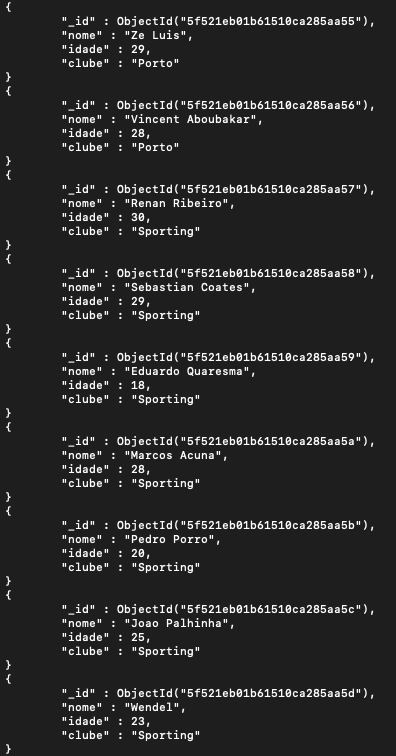
\includegraphics[width=.4\linewidth,height = 10cm]{jogadores3.png}}}
  \qquad
  \subfloat{{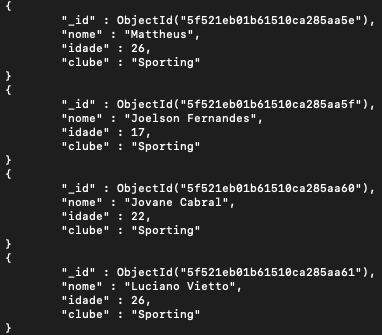
\includegraphics[width=.4\linewidth,height=5cm]{jogadores4.png}}}
  
  \caption {Documentos relativos aos jogadores}

  \label{fig:povoamento}
\end{figure}


\begin{figure}[H]

  \centering
  \captionsetup{justification=centering}

  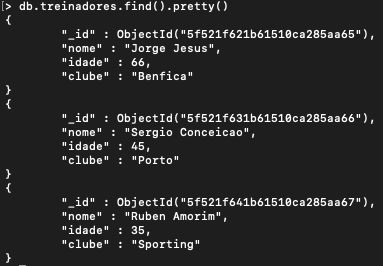
\includegraphics[width = 0.8\textwidth]{treinadores.png}
  
  \caption {Documentos relativos aos treinadores}

  \label{fig:povoamento}
\end{figure}









